\documentclass[12pt]{article}
%	options include 12pt or 11pt or 10pt
%	classes include article, report, book, letter, thesis

% \usepackage[margin=0.75in]{geometry}
\usepackage[margin=0.5in]{geometry}
\setlength{\parindent}{0pt}

\usepackage{hyperref}

%for writing of code in blocks like
%\begin{lstlisting}
%   .......
%\end{lstlisting}
\usepackage{listings}
\usepackage{color}
\usepackage{enumitem}
\usepackage{graphicx}

\definecolor{dkgreen}{rgb}{0,0.6,0}
\definecolor{gray}{rgb}{0.5,0.5,0.5}
\definecolor{mauve}{rgb}{0.58,0,0.82}

\lstset{frame=tb,
  language=C++,
  aboveskip=3mm,
  belowskip=3mm,
  showstringspaces=false,
  columns=flexible,
  basicstyle={\small\ttfamily},
  numbers=none,
  numberstyle=\tiny\color{gray},
  keywordstyle=\color{blue},
  commentstyle=\color{dkgreen},
  stringstyle=\color{mauve},
  breaklines=true,
  breakatwhitespace=true,
  tabsize=3
}
%%%%%%%%%%%%%%%%%%%%%%

\title{Life of a Particle : Quiz 3}
\author{Sam Meehan \& Claire David}
\date{Due Date : 31 January 2019}

\begin{document}
\maketitle
\vspace{-3ex}
\textbf{Guidelines}:
\newline
This quiz will last 15 minutes. Write your answers on paper explaining how you get to the results. 

\section{The unit of charge: the Coulomb}
The elementary charge carried by the electron is $q_e = 1.6021766208(98) \times 10^{-19}$ C.\\
Do you know intuitively what is the charge in one Coulomb?

\begin{figure}[h]
    \centering
    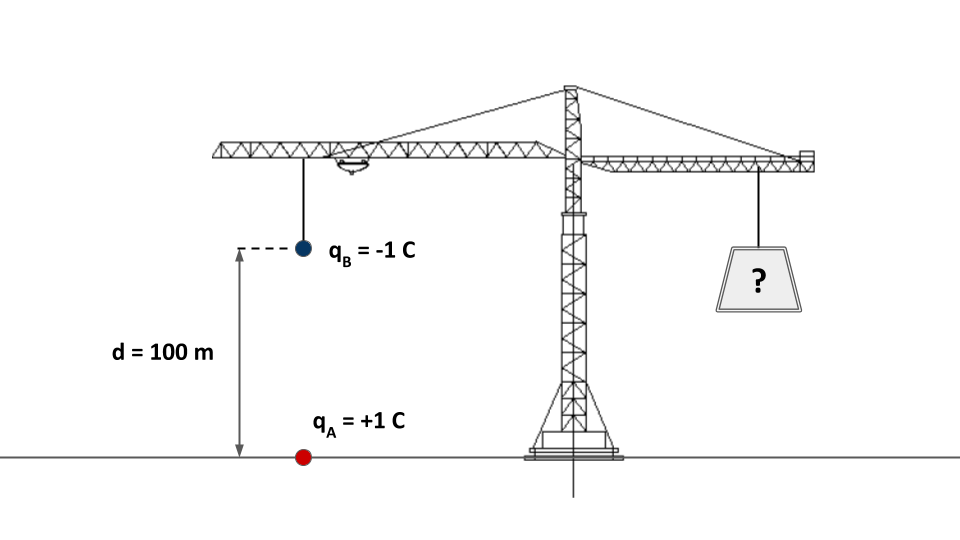
\includegraphics[width=0.8\textwidth]{Coulomb_quiz.png}
%     \caption{}
%     \label{fig:mesh1}
\end{figure}
Imagine that we can fix a positive charge A of one Coulomb in the ground. Let's have a crane where we hang a negative charge B of one Coulomb above the first at a distance $d = 100$ m. The two charges will attract each other, according to the Coulomb force.\\

\textbf{Question A:} What is the mass to be suspended on the other side of the crane to balance this system out? Compare this to a day-to-day life object.\\

\textbf{Question B:} A typical lightning strike is about 40 coulombs of charge, consisting of separate "strokes" (that's why lightning usually looks flickery). Each stroke lasts about 30 microseconds. What is the current?\\

\textit{Reminders on next page (there is also a second question!)}\\
\newpage
Coulomb's law is given by:
\begin{equation}
 \mathbf{F_{12}} = k_e \frac{q_1 \, q_2}{| \, \mathbf{r_{21}}|^2} \: \mathbf{\hat{r}_{21}} 
\end{equation}
with:
    \begin{description}
        \item $k_e$: Coulomb's constant, $k_e = 8.9875517873681764 \times 10^9$ N m$^2$ C$^{-2}$
        \item $q_i$: charge of object $i$
        \item $r$: distance between the charges
    \end{description}

\section{The electron volt}
An electron volt (eV) is the energy an electron gains when it is accelerated through a potential difference of one volt. 
This unit of energy is commonly used in subatomic physics. One electron volt corresponds to 1.60218  $ \cdot 10^{-19}$ Joules. \\

A Kingsbite Milk Chocolate Bar has 274 Calories (one dietary Calorie is 1000 calories, or 4184 Joules).\\

The LHC operates at 14 TeV (tera electron volts, or 10$^{12}$ eV).\\


\textbf{Question A:} How does the energy of the proton-proton collisions at LHC compare with respect to the energy stored in a Kingsbite Milk Chocolate Bar?\\ 

\textbf{Question B:} Make the same comparison with energy density.\\

\vspace{4ex}
\hrule
\vspace{4ex}
\textit{Guidelines on input data:} as volumes you can use these estimations:
    \begin{description}
        \item LHC: a proton has a volume of roughly 1 fm$^3$, or about 10$^{-39}$ cm$^3$
        \item Kingsbite Milk Chocolate Bar is about 10 cm $\times$ 1/2 cm $\times$ 20 cm = 100 cm$^3$
    \end{description}

\vspace{4ex}
\hrule
\vspace{4ex}
    
\end{document}